\documentclass[11pt, oneside]{article}
\usepackage[letterpaper, margin=2cm]{geometry}
\usepackage{MATH667}
\usepackage{booktabs}

\begin{document}
\noindent \textbf{\Large{Caleb Logemann \\
MATH667 Hyperbolic Partial Differential Equations \\
Homework 5
}}

%\lstinputlisting[language=MATLAB]{H01_23.m}
\begin{enumerate}
  \item % #1 Done
    For the following schemes to solve nonlinear conservation laws, show which
    ones are monotone schemes.
    \begin{itemize}
      \item Godunov scheme \hfill \\ % Done
        The Godunov scheme is monotone if the CFL condition is met.
        To see this note that the Godunov method can be written as
        $U^{n+1}_j = H(U^n_{j-1}, U^n_j, U^n_{j-1})$ where
        \[
          H(U_{j-1}, U_j, U_{j+1}) = U_j - \frac{\Delta t}{\Delta x}\p{F_{j+1/2} - F_{j-1/2}}
        \]
        and
        \begin{align*}
          F_{j+1/2} &=
          \begin{cases}
            \min[u \in \br{U_{j}, U_{j+1}}]{f(u)} & U_{j} \le U_{j+1} \\
            \max[u \in \br{U_{j+1}, U_{j}}]{f(u)} & U_{j} > U_{j+1}
          \end{cases} \\
          F_{j-1/2} &=
          \begin{cases}
            \min[u \in \br{U_{j-1}, U_{j}}]{f(u)} & U_{j-1} \le U_{j} \\
            \max[u \in \br{U_{j}, U_{j-1}}]{f(u)} & U_{j-1} > U_{j}
          \end{cases}
        \end{align*}
        To show that this method is monotone, we need to show that
        $\pd{H}{U_i} \ge 0$ for $i = j-1, j, j+1$.

        First consider $\pd{H}{U_{j-1}}$.
        \begin{align*}
          \pd{H}{U_{j-1}} &= \frac{\Delta t}{\Delta x} \pd{F_{j-1/2}}{U_{j-1}}
        \end{align*}
        Now consider $\pd{F_{j-1/2}}{U_{j-1}}$.
        If $U_{j-1} \le U_{j}$ and $U_{j-1}$ increases the size of
        $\br{U_{j-1}, U_j}$ decreases.
        Now we are taking a minimum over a smaller integral so the value of
        $F_{j-1/2}$ increases.
        If $U_{j-1} > U_{j}$ and $U_{j-1}$ increases then the size of
        $\br{U_j, U_{j-1}}$ increases.
        Now the value of $F_{j-1/2}$ would increase as we are taking a maximum
        over a larger interval.
        This implies that $\pd{F_{j-1/2}}{U_{j-1}} \ge 0$.
        This shows that
        \[
          \pd{H}{U_{j-1}} \ge 0.
        \]

        Now consider $\pd{H}{U_{j+1}}$.
        \begin{align*}
          \pd{H}{U_{j+1}} &= -\frac{\Delta t}{\Delta x} \pd{F_{j+1/2}}{U_{j+1}}
        \end{align*}
        Now consider $\pd{F_{j+1/2}}{U_{j+1}}$.
        If $U_{j} \le U_{j+1}$ and $U_{j+1}$ increases the size of
        $\br{U_{j}, U_{j+1}}$ increases.
        Now we are taking a minimum over a larger integral so the value of
        $F_{j+1/2}$ possibly decreases.
        If $U_{j} > U_{j+1}$ and $U_{j+1}$ increases then the size of
        $\br{U_{j+1}, U_{j}}$ decreases.
        Now the value of $F_{j+1/2}$ would increase as we are taking a maximum
        over a larger interval.
        This implies that $\pd{F_{j+1/2}}{U_{j+1}} \le 0$.
        This shows that
        \[
          \pd{H}{U_{j+1}} \ge 0.
        \]

        Last consider $\pd{H}{U_j}$.
        \begin{align*}
          \pd{H}{U_{j+1}} &= 1 - \frac{\Delta t}{\Delta x}\p{\pd{F_{j+1/2}}{U_{j}} - \pd{F_{j-1/2}}{U_j}}
        \end{align*}
        I will first consider $\pd{F_{j+1/2}}{U_j}$ and $\pd{F_{j-1/2}}{U_j}$.
        Note that if $U_j$ increases the value of $F_{j+1/2}$ may increase because
        either the interval over which a minimum is being taken will decrease
        of the intervale over which a maximum is being taken will increase.
        However this increase is bounded by $\alpha = \max{\abs{f'(u)}}$ the
        global maximum of the wave speed.
        So
        \[
          \pd{F_{j+1/2}}{U_j} \le \alpha
        \]
        Similarly for $F_{j-1/2}$.
        If $U_j$ increases then $F_{j-1/2}$ may decrease but it is bounded below
        by $-\alpha$.
        So
        \[
          \pd{F_{j-1/2}}{U_j} \ge -\alpha.
        \]
        Therefore
        \begin{align*}
          \pd{H}{U_{j+1}} &\ge 1 - \frac{2\Delta t}{\Delta x} \alpha
        \end{align*}
        So if the following CFL condition is met, then the Godunov method is monotone.
        \[
          \frac{\Delta t \alpha}{\Delta x} < \frac{1}{2}
        \]

      \item Lax-Friedrichs scheme \hfill \\ % Done
        The Lax-Friedrichs scheme is monotone if the CFL condition is met.
        To see this note that the Lax-Friedrichs method can be written as
        $U^{n+1}_j = H(U^n_{j-1}, U^n_j, U^n_{j-1})$ where
        \[
          H(U_{j-1}, U_j, U_{j+1}) = \p{1 - \frac{\alpha \Delta t}{\Delta x}} U_j
          + \frac{\alpha \Delta t}{2 \Delta x} \p{U_{j+1} + U_{j-1}}
          - \frac{\Delta t}{2 \Delta x} \p{f(U_{j+1}) - f(U_{j-1})}
        \]
        and $\alpha = \max[u]{\abs{f'(u)}}$
        To show that this method is monotone, we need to show that
        $\pd{H}{U_i} \ge 0$ for $i = j-1, j, j+1$.

        First consider $\pd{H}{U_j}$.
        \begin{align*}
          \pd{H}{U_j} &= \p{1 - \frac{\alpha \Delta t}{\Delta x}} \\
          \p{1 - \frac{\alpha \Delta t}{\Delta x}} &\ge 0 \\
          1 &\ge \frac{\alpha \Delta t}{\Delta x} \\
        \end{align*}
        This is exactly the CFL condition, so this condition is satisfied by this method.

        Second consider $\pd{H}{U_{j-1}}$.
        \begin{align*}
          \pd{H}{U_{j-1}} &= \frac{\alpha \Delta t}{2 \Delta x} + \frac{\Delta t}{2 \Delta x} f'(U_{j-1}) \\
          &= \frac{\Delta t}{2 \Delta x}\p{\alpha + f'(U_{j-1})}
          \intertext{Since $\alpha = \max[u]{\abs{f'(u)}} \ge f'(U_{j-1})$, then
            $\p{\alpha + f'(U_{j-1})} \ge 0$ and}
          \pd{H}{U_{j-1}} &\ge 0
        \end{align*}

        Finally consider $\pd{H}{U_{j+1}}$.
        \begin{align*}
          \pd{H}{U_{j+1}} &= \frac{\alpha \Delta t}{2 \Delta x} - \frac{\Delta t}{2 \Delta x} f'(U_{j+1}) \\
          &= \frac{\Delta t}{2 \Delta x}\p{\alpha - f'(U_{j+1})}
          \intertext{Since $\alpha = \max[u]{\abs{f'(u)}} \ge f'(U_{j-1})$, then
            $\p{\alpha - f'(U_{j+1})} \ge 0$ and}
          \pd{H}{U_{j+1}} &\ge 0
        \end{align*}

        These three conditions are met by the Lax-Friedrichs method, so the scheme is monotone.

      \item Local Lax-Friedrichs scheme \hfill \\ % Done
        The Local Lax-Friedrichs scheme is monotone if the CFL condition is meet.
        To see this note that the Local Lax-Friedrichs method can be written as
        $U^{n+1}_j = H(U^n_{j-1}, U^n_j, U^n_{j-1})$ where
        \[
          H(U_{j-1}, U_j, U_{j+1}) = \p{1 - \frac{\p{\alpha_+ + \alpha_-} \Delta t}{2\Delta x}} U_j
          + \frac{\Delta t}{2 \Delta x} \p{\alpha_+ U_{j+1} + \alpha_- U_{j-1}}
          - \frac{\Delta t}{2 \Delta x} \p{f(U_{j+1}) - f(U_{j-1})}
        \]
        and $\alpha_+ = \max[\p{U_j, U_{j+1}}]{\abs{f'(u)}}$ and $\alpha_- = \max[\p{U_j, U_{j-1}}]{\abs{f'(u)}}$.
        To show that this method is monotone, we need to show that
        $\pd{H}{U_i} \ge 0$ for $i = j-1, j, j+1$.

        First consider $\pd{H}{U_j}$.
        \begin{align*}
          \pd{H}{U_j} &= \p{1 - \frac{\p{\alpha_+ + \alpha_-} \Delta t}{2\Delta x}} \\
          \p{1 - \frac{\p{\alpha_+ + \alpha_-} \Delta t}{2\Delta x}} &\ge 0 \\
          1 &\ge \frac{\p{\alpha_+ + \alpha_-} \Delta t}{2\Delta x} \\
        \end{align*}
        Since $\alpha_+$ and $\alpha_-$ are both less than $\alpha$, this
        condition is met if the CFL condition is met.

        Second consider $\pd{H}{U_{j-1}}$.
        \begin{align*}
          \pd{H}{U_{j-1}} &= \frac{\alpha_- \Delta t}{2 \Delta x} + \frac{\Delta t}{2 \Delta x} f'(U_{j-1}) \\
          &= \frac{\Delta t}{2 \Delta x}\p{\alpha_- + f'(U_{j-1})}
          \intertext{Since $\alpha_- = \max[\br{U_{j-1}, U_j}]{\abs{f'(u)}} \ge f'(U_{j-1})$, then
            $\p{\alpha_- + f'(U_{j-1})} \ge 0$ and}
          \pd{H}{U_{j-1}} &\ge 0
        \end{align*}

        Finally consider $\pd{H}{U_{j+1}}$.
        \begin{align*}
          \pd{H}{U_{j+1}} &= \frac{\alpha_+ \Delta t}{2 \Delta x} - \frac{\Delta t}{2 \Delta x} f'(U_{j+1}) \\
          &= \frac{\Delta t}{2 \Delta x}\p{\alpha_+ - f'(U_{j+1})}
          \intertext{Since $\alpha = \max[\br{U_j, U_{j+1}}]{\abs{f'(u)}} \ge f'(U_{j-1})$, then
            $\p{\alpha_+ - f'(U_{j+1})} \ge 0$ and}
          \pd{H}{U_{j+1}} &\ge 0
        \end{align*}

        These three conditions are met by the Local Lax-Friedrichs method, so the scheme is monotone.

      \item Lax-Wendroff scheme \hfill \\ % Done
        The Lax-Wendroff scheme is not monotone.
        This is obvious because the Lax-Wendroff scheme is second order and
        monotone schemes must be first order at most.
        Also Lax-Wendroff creates oscillations at shocks, which are clearly not
        monotone.

        To see this specifically, consider $f(u) = u$.
        In this case,
        \[
          H(U_{j-1}, U_j, U_{j+1}) = U_j - \frac{\Delta t}{2\Delta x} \p{U_{j+1} - U_{j-1}}
          + \frac{\Delta t^2}{2 \Delta x^2} \p{U_{j+1} - 2U_j + U_{j-1}}
        \]
        Now consider $\pd{H}{U_{j+1}}$
        \begin{align*}
          \pd{H}{U_{j+1}} &= -\frac{\Delta t}{2\Delta x} + \frac{\Delta t^2}{2 \Delta x^2} \\
          &= \frac{\Delta t}{2\Delta x}\p{\frac{\Delta t}{\Delta x} - 1} \\
          &\le 0 \\
        \end{align*}
        If the CFL condition is satisfied then
        $\p{\frac{\Delta t}{\Delta x} - 1} \le 0$, so this partial
        derivative is negative and the method is not monotone.
    \end{itemize}

  \item % #2 Done
    Solve Burger's equation $u_t + \p{\frac{u^2}{2}}_x = 0$ on
    $x \in \br{0, 2\pi}$ with initial data $u(x, 0) = 1 + \frac{1}{2} \sin{x}$.
    Let's consider the 1\textsuperscript{st} order finite difference Godunov scheme.
    Implement the scheme to (a) $t = 1.0$ and (b) $t = 3.0$.
    Apply periodic boundary conditions.
    For part (a) output $L^{\infty}$ error/order table with uniform mesh
    $N = 20, 40, 80, 160$.
    For part (b) graph the simulation with $N = 80$ and solid line for exact
    solution and symbols for numerical approximations.

    The following is my implementation of the Godunov scheme.
    \lstinputlisting[language=MATLAB]{godunov.m}
    \begin{enumerate}
      \item[(a)] % Done
        The following script uses this method to compute the solutions at
        $t = 1.0$ for the different values of $N$ and it shows the order of
        convergence.
        \lstinputlisting[language=MATLAB, lastline=32]{H05.m}
        The following table is output from this script.
        Note that the Godunov method converges with order 1, which is what we
        expect.
        \begin{center}
          \begin{tabular}{*{5}{c}}
            \toprule
            N & $\Delta x$ & $L^{\infty}$ Error & Order \\
            \midrule
            20.000 & 0.314 & 0.098 & - \\
            40.000 & 0.157 & 0.049 & 0.997 \\
            80.000 & 0.079 & 0.025 & 0.987 \\
            160.000 & 0.039 & 0.013 & 0.980 \\
            \bottomrule
          \end{tabular}
        \end{center}

      \item[(b)] % Done
        The following script uses the Godunov method to plot the solution
        at $t = 3.0$.
        \lstinputlisting[language=MATLAB, firstline=34]{H05.m}
        The following image is produced.
        \begin{center}
          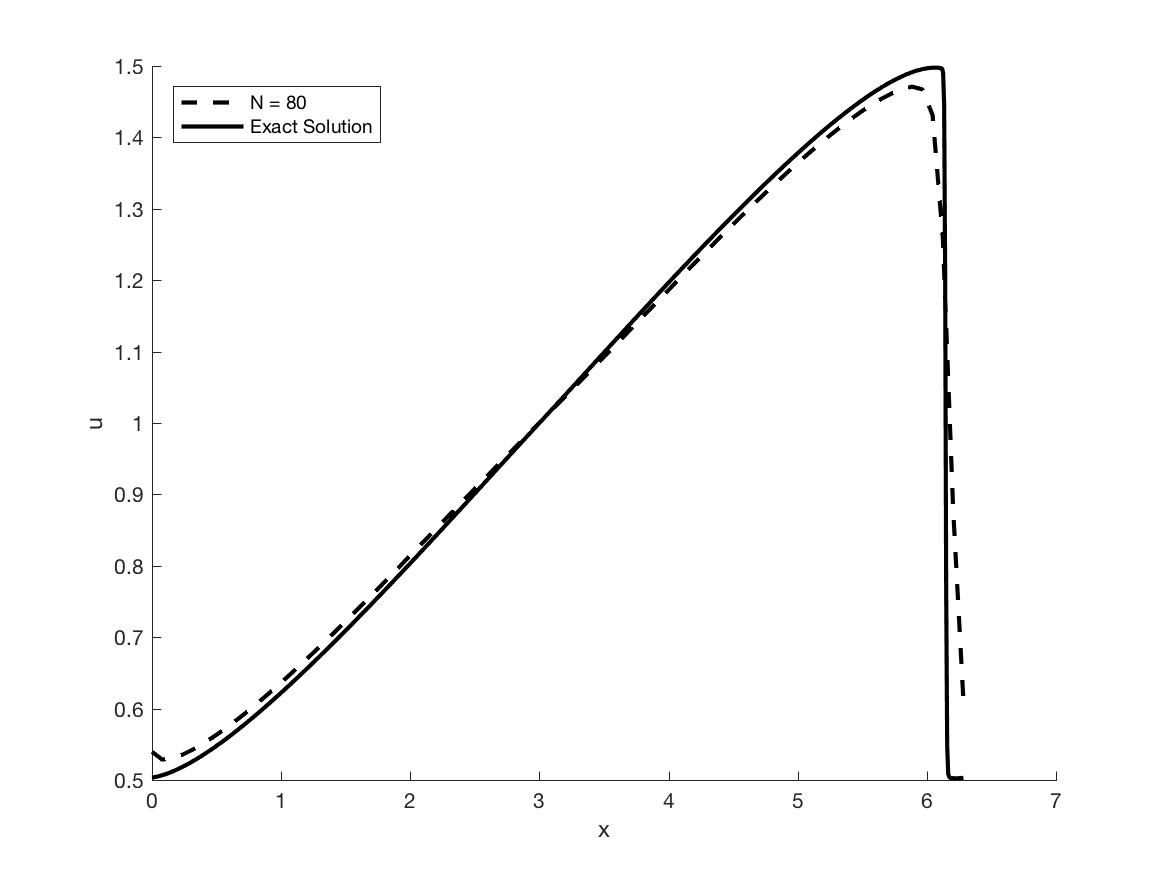
\includegraphics[scale=0.7]{Figures/05_01.png}
        \end{center}
    \end{enumerate}
\end{enumerate}
\end{document}
